\documentclass[a4paper,12pt]{article}
\renewcommand{\baselinestretch}{1.5}
\usepackage{amsmath}
%\usepackage{cite}
\usepackage[hidelinks]{hyperref}
\usepackage{geometry}
\usepackage{subcaption}
\usepackage{graphicx}
\usepackage{booktabs} 
\usepackage{multirow}
\usepackage{siunitx}
\usepackage{natbib}
\usepackage{url}
\usepackage[english]{babel}
\usepackage{blindtext}
\usepackage[table,xcdraw]{xcolor}
\usepackage[format=hang,font=small,labelfont=bf]{caption}
\usepackage[hang,flushmargin]{footmisc} 


\usepackage{fancyhdr}
\pagestyle{fancy}
\lhead{}


\geometry{left=30mm,right=30mm,top=35mm,bottom=30mm,headheight=15pt}

\graphicspath{{./img/}}


\begin{document}
	
	\begin{titlepage}
		\centering
		\begin{figure}[!h]
			\centering
			
\includegraphics[width=0.5\textwidth]{UZH}
		\end{figure}
		\Large{\textbf{The Effect of U.S. Real
        GDP on different S\&P500 sector indices' market capitalizations}\\}

		\vfill
		\vfill
		\vfill
  
		
		\normalsize{Naomi Huser, 17-056-201 \\
                    Jonas Neller, 21-730-676 \\ 
				Lorena Tassone, 18-700-237
                }
		
		\vfill
			
		\normalsize{December 19, 2022}
		
		\vfill
		\vfill
	
		\normalsize{Department of Banking \& Finance \\ Digital Tools for Finance \\ Dr. Igor Pozdeev \\ }
	
		\vfill
        \begin{abstract}
            This paper analyses the effect of the United States Real GDP on the average sector-specific market capitalization of companies listed in the  S\&P 500 index between 2007 and 2021 by means of a regression analysis. We show that a stable positive relationship exists within the Communications and Real Estate sectors.
			
			\vspace{3mm}
			
			\textbf{Keywords:} Factor Timing, Practical Implication, Investment Strategy
		\end{abstract}
		
		
	\end{titlepage}
	


	\tableofcontents

	\clearpage
	\listoffigures
	
	\clearpage
	\listoftables
	
	\clearpage


 \section{Introduction}
	\vspace{1cm}
One of the most discussed and theoretically as well as empirically studied question in economics seems to be the possibility of macroeconomic factors significantly affecting the stock market and its prices.\\
As activities on the financial markets play an essential role in the everyday life of individual households, detecting a relationship between movements in the markets and specific macroeconomic elements is a topic, which has been occupying many researchers in the fields of finance and economics.\\
Multiple literature pieces attempting to describe a significant pattern in order to clear up parts of the uncertainties ruling the financial markets have been published so far. However, it seems that the search for clear answers to the crucial question as old as the stock markets themselves continues.

\noindent A strongly related issue, posing an interesting and notable further question would be the influence of particular macroeconomic factors on the market capitalisation of companies listed in key indices such as the S\&P500 Index.\\
As market capitalisation is calculated by multiplying the total number of outstanding stocks of a company by their price, it is directly linked to the prices on the financial markets.
\begin{equation}
  Market Cap = Current Share Price * Total Number of Shares Outstanding  
\end{equation}

\noindent Thus, analysing the effect of individually chosen macroeconomic factors such as the U.S. Real Gross Domestic Product on the market capitalisation of companies traded in the S\&P500 is closely connected to studies on the question discussing the influence of macroeconomic factors on the stock markets.

\clearpage
\section{Research Question}

The main purpose of this paper is to establish a credible answer to the following research question:

\bigskip

\noindent "What is the effect of U.S. Real GDP on different S\&P500 sector indices' market capitalization"

\bigskip

\noindent This purpose will be achieved through regression analysis, the contents of various literature pieces as well as the knowledge and skills of the writers. The Macroeconomic Factor most essential in this paper will therefore be the Real Gross Domestic Product of the United States. However, as mentioned in the introductory paragraph having a look at multiple other economically significant factors would most likely prove beneficial and an interesting study. Thus, an additional focus beyond U.S. Real GDP will be seen throughout this paper as well.


\clearpage
\section{Data}

The Data used for the regression analysis will be in the form of quarterly panel data from the year 2007 until 2021 and retrieved from Bloomberg and from the Federal Reserve Economic Research database (FRED). The Data includes level values of:

\begin{itemize}
  \item Market Capitalization of S\&P500 Index constituent in Million U.S. Dollar for different sectors \footnote{As an approximation of the index, we used the constituents of the iShares Core S\&P 500 UCITS ETF.}
  \item United States Real Gross Domestic Product in Million U.S. Dollar
  \item United States Unemployment Rate in Percentage Points
  \item United States Federal Debt in Million U.S. Dollar
  \item United States Federal Rate in Percentage Points
  \item United States Crude Prices in U.S. Dollar
\end{itemize}

\noindent The market capitalization of individual companies in the S\&P500 Index will be sectioned into the following sectors:\\
Communication, Consumer Discretionary, Consumer Staples, Energy, Financials, Health Care, Industrials, Information Tech, Materials, Real Estate, and Utilities.

\noindent The mean value of the sector-specific market capitalization per quarter will then be calculated and used as the final form of the dependent variable in the regression analysis. Missing data occurring from the market capitalization dataset will be dealt with by removing individual companies with missing values completely.

\noindent The programming will be executed in the programming language "Python".

\clearpage
\section{Regression Variables}

We employ four macroeconomic factors as Control Variables in our regression model. These factors will not only be included to control for the omitted variable bias but also to have a look at macroeconomic factors beyond the real GDP as mentioned above. They will thus present the focus of the regression analysis in order to ultimately answer the leading question.

\subsection{Real GDP}

It is well known that one of the most studied questions in the realm of financial markets is whether or not there exist macroeconomic factors, which influence stock markets in a significant manner.
Well-studied and analysed factors include the GDP \citep{pilinkus2009short}.

\noindent As the GDP affects the stock market and prices, it will influence other elements such as the market capitalisation of publicly traded companies, for instance, the companies included in the S\&P500 Index \citep{pilinkus2009short}.

\subsection{Unemployment Rate}

As the unemployment rate can serve as an indicator of the economy’s state, a decrease in the rate can lead to an increase in investments \citep{Forbes2022}.

\noindent A lower unemployment rate signals a healthier economy with higher production. This scenario would result in more enthusiasm from investors and thus expand investments \citep{Forbes2022}. Therefore, following this theory the macroeconomic factor “Unemployment Rate” is expected to have a significant impact on the market capitalisation of publicly traded companies.

\subsection{Crude Prices}

It is theoretically stated, that an increase in oil prices will most likely result in dampened economic growth, which can lead to decreased expected company earnings, followed by a negative effect on stock prices \citep{ECB2004}.

\noindent Additionally, higher input prices for companies caused by increased oil prices can lead to compressed profit margins. 
These factors in combination with the uncertainty increased prices create are likely to cause a negative significant effect on variables such as market capitalizations of publicly traded companies \citep{ECB2004}.

\subsection{Federal Debt Level}

An essential element of growth and increased economic productivity is a strong fiscal outlook \citep{PGPF2022}.

\noindent Increased public debt is most likely to result in increased government spending on interest rates and thus less on public investment, leading to decreased access to capital, resources for future public and private investments as well as confidence in the prospective economic state \citep{PGPF2022}.\\
Thus, a significant negative effect of increased federal debt on elements such as market capitalizations of publicly traded companies is to be expected.

\subsection{Federal Rate}

As the Federal Funds Rate greatly influences other rates such as the prime interest rate, mortgage loan rates and credit card annual percentage rates, it is of importance in the borrowing and lending activities of various corporations and consumers in the economy \citep{Hall2022}.

\noindent An increase in the Federal Funds Rate leads to increased borrowing costs for companies and consumers. This will result in heightened prices, which will discourage consumer spending. Lower spending will create lower revenues and profits, which ultimately negatively impacts the stock prices of the affected firms and therefore their market capitalization \citep{Hall2022}.



\clearpage
\section{Regression Model}

\noindent The Regression Model used in this paper to analyse the effect of U.S. real GDP and other macroeconomic factors on the sector-specific average market capitalization of companies listed in the S\&P500 Index will be in the form of a multiple linear regression model:
\begin{equation}
  Y_t^{sector}= \beta_0 + \beta_1 X_{1,t} + \beta_2 X_{2,t} + \beta_3 X_{3,t} + \beta_4 X_{4,t} + \beta_5 X_{5,t} + u_t 
\end{equation}

\noindent As in any regression model, $Y_t$ represents the dependent variable also known as the regressand, whose expected values are estimated with the use of the independent variables known as regressors. 
In this model the regressors are denoted as $X_{it}$.\\
The $\beta_i$ portrays the coefficients. These are the estimated values for the relationship between the regressors and the regressand and thus of great interest and the main focus throughout the regression analysis.

\begin{table}[htbp]
\centering 
\setlength\tabcolsep{4pt}
\newcommand\hd[1]{\multicolumn{1}{c}{\textit{#1}}}

\caption{Variable Description}

\begin{tabular}{ c c c } \hline\hline
\hd{Variable in Model} & \hd{Representative for}  & \hd{Label in Python} \\ \hline\hline
$Y_t^{sector}$ & Average Sector Market Capitalization &mean$\_$\textit{sector} \\ \hline
$X_{1,t}$ & U.S. Real GDP &Real$\_$GDP \\ \hline
$X_{2,t}$ &U.S. Unemployment Rate &Unemployment$\_$rate \\ \hline
$X_{3,t}$ &U.S. Crude Prices & Crude$\_$price \\ \hline
$X_{4,t}$ &U.S. Federal Debt & Federal$\_$debt \\ \hline
$X_{5,t}$ &U.S. Federal Rate & Federal$\_$rate \\ \hline
$\beta_0$ &Constant &- \\ \hline
$\beta_1$ &Coefficient of U.S. Real GDP &- \\ \hline
$\beta_2$ &Coefficient of U.S. Unemployment Rate &- \\ \hline
$\beta_3$ &Coefficient of U.S. Crude Prices &- \\ \hline
$\beta_4$ &Coefficient of U.S. Federal Debt &-\\ \hline
$\beta_5$ &Coefficient of U.S. Federal Rate &-\\ \hline
$u_t$  &Error Term &- \\ \hline

\hline
\end{tabular}
\end{table}

\clearpage

\section{Empirical Analysis}

Tables 1 and 2 on page 13 list the regression outputs, which have been estimated in python.
In the following, there will be five sections each describing the outputs and general inference on the effects of U.S. Real GDP, U.S. Unemployment Rate, U.S. Crude Prices, U.S. Federal Debt and U.S. Federal Rate on average Market Capitalization over time by sectors. In the Appendix, the regression and residual plots of all sectors for which regressions have been run can be found as well as a heatmap depicting the correlations between the macroeconomic indicators used as control variables in the regressions.

\subsection{U.S. Real GDP}

Statistically significant estimations of the coefficient for U.S. Real GDP $\beta_1$ can be observed for the sectors Communication and Real Estate. The parameter for the communication sector has a value of 0.0260 and is significant at the 1$\%$ level. The standard error is 0.0094 and the adjusted coefficient of determination ${R}^2$ has a value of 0.9640. An increase of one unit of real GDP, which would be equal to 1 Million U.S. Dollars, thus is estimated to lead to an increase of the average market capitalization by 26 Thousand U.S. Dollars. The parameter for the real estate sector has a value  of 0.0019 and is significant at the 5$\%$ level. The standard error is 0.0009 and the adjusted coefficient of determination ${R}^2$ has a value of 0.9795. An increase of one unit of real GDP thus is estimated to lead to an increase of the average market capitalization by 1.9 Thousand U.S. Dollars. Thus, for both sectors Communication and Real Estate, a positive statistically significant effect on average market capitalization can be estimated. The influence of U.S. real GDP on average market capitalization in the other sectors seems to be statistically insignificant.

\subsection{U.S. Unemployment Rate}


Statistically significant estimations of the coefficient for U.S. Unemployment Rate $\beta_2$ are to be seen for the sectors Consumer Staples, Energy, Industrials and Real Estate. The parameter for the consumer staples sector has a value of -1996.1013 and is significant at the 1$\%$ level. The standard error is 475.0441 and the adjusted coefficient of determination ${R}^2$ has a value of 0.9573.\\ An increase of one percentage point in the unemployment rate thus is estimated to lead to a decrease of the average market capitalization by 1996.1013 Million U.S. Dollars. Similarly, statistically significant negative effects of the unemployment rate on average market capitalization can be estimated for the sectors Energy, Industrials and Real Estate ranging from values of -370.1013 to -4172.2230 with the lowest significance level being at 5$\%$. The standard errors lie between 178.3417 and 1072.6771. The lowest adjusted coefficient of determination ${R}^2$ can be seen in the energy sector with a value of 0.6989. The influence of the U.S. unemployment rate on average market capitalization in the remaining sectors seems to be statistically insignificant.

\subsection{U.S. Crude Prices}

We receive statistically significant estimations of the coefficient for the U.S. Unemployment Rate $\beta_3$ for the sectors Communication, Energy, Health Care, Industrials and Materials. The parameter for the communication sector has a value of -225.7810 and is significant at the 1$\%$ level. The standard error is 69.5862 and the adjusted coefficient of determination ${R}^2$ has a value of 0.9640. An increase of crude oil prices by one unit thus leads to a decrease of the average market capitalization by 225.7810 Million U.S. Dollars. Similarly, a statistically significant negative effect of crude prices on average market capitalization can be estimated for the sector Health Care at the 1$\%$ level with a value of -51.3752 and a standard error of 18.6742. The adjusted coefficient of determination ${R}^2$ has a value of 0.9657. Contrary, a statistically significant positive influence can be estimated for the sectors Energy, Industrials and Materials ranging from values 34.4213 to 293.3256 with the lowest significance level being at 1$\%$. The standard errors lie between 7.7025 and 39.8019. The lowest adjusted coefficient of determination ${R}^2$ can be seen in the energy sector with a value of 0.6989. The influence of U.S. crude prices on average market capitalization in the remaining sectors are statistically insignificant.

\subsection{U.S. Federal Debt}

Statistically significant estimations of the coefficient for U.S. Federal Debt $\beta_4$ are to be seen for all the sectors except Energy and Financials. The parameter for the communication sector has a value of 0.0042 and is significant at the 10$\%$ level. The standard error is 0.0022 and the adjusted coefficient of determination ${R}^2$ has a value of 0.9640. An increase of the federal debt level by one unit, which would be equal to 1 Million U.S. Dollars, thus is estimated to lead to an increase of the average market capitalization by 4.2 Thousand U.S. Dollars. Similarly, a statistically significant positive effect of the federal debt level can be estimated for the other sectors ranging from values of 0.0007 to 0.003 with the lowest significance level being at 1$\%$. The standard errors lie between 0.0002" and 0.0023. The lowest adjusted coefficient of determination ${R}^2$ can be seen in the energy sector with a value of 0.8754.



\subsection{U.S. Federal Rate}


Statistically significant estimations of the coefficient for U.S. Federal Funds Rate $\beta_5$ is to be seen for all the sectors except Energy. The parameter for the communication sector has a value of 6599.3047 and is significant at the 1$\%$ level. The standard error is 1593.9435 and the adjusted coefficient of determination ${R}^2$ has a value of 0.9640. An increase of the federal debt level by one percentage point thus is estimated to lead to an increase of the average market capitalization by 6599.3047 Million U.S. Dollars. Thus, a positive statistically significant effect on average market capitalization can be estimated. Similarly, a statistically significant positive effect of the federal rate can be estimated for the other sectors ranging from values of 375.9451 to 8851.4555 with the lowest significance level being at 5$\%$. The standard errors lie between 151.5784 and 1683.2421. The lowest adjusted coefficient of determination ${R}^2$ can be seen in the energy sector with a value of 0.8754.

\clearpage

\begin{table}
\caption{Regression Output (1/2)}
\label{}
\begin{center}
\tiny
\begin{tabular}{lllllll} \hline                  & Communication & Consumer Discretionary & Consumer Staples & Energy  & Financials  \\  \hline 
Intercept          & -426623.1332***     & -101575.6982*      & 63161.7972*        & 140636.6070*  & -61152.2646    \\                    & (131825.8134)       & (53595.7324)       & (33392.2623)       & (75401.6600)  & (49080.7712)     \\  
Real GDP          & 0.0260***           & 0.0049             & -0.0031            & -0.0054       & 0.0053          \\                   & (0.0094)            & (0.0038)           & (0.0024)           & (0.0053)      & (0.0035)           \\  
Unemployment rate & 1384.5260           & 345.4589           & -1996.1013***      & -4172.2230*** & -1083.2989        \\                    & (1875.3769)         & (762.4622)         & (475.0441)         & (1072.6771)   & (698.2316)        \\  
Crude price       & -225.7810***        & 10.8616            & -26.0573           & 293.3256***   & 4.1270   \\                    & (69.5862)           & (28.2913)          & (17.6266)          & (39.8019)     & (25.9080)    \\ 
Federal debt      & 0.0042*             & 0.0025***          & 0.0030***          & 0.0009        & 0.0011        \\                   & (0.0022)            & (0.0009)           & (0.0006)           & (0.0013)      & (0.0008)        \\ 
Federal rate      & 6599.3047***        & 3160.2254***       & 959.3995**         & -923.9504     & 2118.2440***    \\                    & (1593.9435)         & (648.0413)         & (403.7554)         & (911.7029)    & (593.4496)     \\ \hline  
R-squared          & 0.9673              & 0.9473             & 0.9611             & 0.7258        & 0.9251         \\  
R-squared Adj.     & 0.9640              & 0.9421             & 0.9573             & 0.6989        & 0.9178         \\ \hline
\end{tabular}
\end{center}
\end{table}

\begin{table}
\caption{Regression Output (2/2)}
\label{}
\begin{center}
\tiny
\begin{tabular}{llllllll}  \hline                    &  Health Care & Industrials & Information Tech. & Materials & Real Estate & Utilities  \\  \hline 
Intercept             & -40738.0436      & 13095.0882        & -100640.4068          & -12439.7112     & -29193.6376**    & -24398.8807      \\                      & (35376.8140)     & (23911.5315)      & (139211.1836)         & (14591.7968)    & (12536.1712)     & (16485.3283)     \\  
Real GDP            & 0.0025           & -0.0006           & 0.0008                & 0.0007          & 0.0019**         & 0.0017           \\                     & (0.0025)         & (0.0017)          & (0.0099)              & (0.0010)        & (0.0009)         & (0.0012)         \\  
Unemployment rate     & -590.8811        & -1244.2789***     & 2037.2711             & -160.3370       & -370.1013**      & -61.4332         \\                        & (503.2767)       & (340.1696)        & (1980.4425)           & (207.5854)      & (178.3417)       & (234.5231)       \\  
Crude price              & -51.3752***      & 34.4213***        & 58.7714               & 38.7420***      & -8.0778          & -7.0955          \\                       & (18.6742)        & (12.6221)         & (73.4847)             & (7.7025)        & (6.6174)         & (8.7020)         \\  
Federal debt            & 0.0022***        & 0.0016***         & 0.0066***             & 0.0007***       & 0.0009***        & 0.0008***        \\                        & (0.0006)         & (0.0004)          & (0.0023)              & (0.0002)        & (0.0002)         & (0.0003)         \\  
Federal rate        & 2100.1269***     & 1395.3062***      & 8851.4555***          & 572.2060***     & 375.9451**       & 1085.0825***     \\                  & (427.7511)       & (289.1211)        & (1683.2421)           & (176.4336)      & (151.5784)       & (199.3288)       \\ \hline  
R-squared           & 0.9688           & 0.9454            & 0.8865                & 0.9273          & 0.9813           & 0.9574           \\   
R-squared Adj.              & 0.9657           & 0.9401            & 0.8754                & 0.9201          & 0.9795           & 0.9532           \\  \hline  \\
\end{tabular}
\end{center}
\end{table}

\clearpage
\section{Conclusion}

The main purpose of this paper was to analyse the effect of United States real GDP on the average sector-specific market capitalization of companies listed in the S\&P500 index over time. Moreover, this paper focused on additional macroeconomic factors of interest such as the Unemployment Rate, Crude Prices, Federal Debt and Federal Funds Rate. 

\noindent Statistically significant positive estimates of the relationship between real GDP and average market capitalization have been evaluated for the Communication and Real Estate sector with respective values of 0.0260 and 0.0019 at the 1$\%$ and 5$\%$ level. Further statistically significant effects have been established for the unemployment rate in the sectors Consumer Staples, Energy, Industrials and Real Estate describing a negative relationship. Crude Prices are estimated to have a statistically significant negative effect in the Health Care sector and a positive effect in the Sectors Energy, Industrials and Materials. The macroeconomic factor Federal Debt is estimated to affect average market capitalization positively on a statistically significant level in all sectors except Energy and Financials. Similarly, for the Federal Funds Rate, a statistically significant positive relationship has been estimated in all sectors except the Energy sector.

\noindent Thus, the answer to the leading question of this paper "What is the effect of U.S. Real GDP on different S\&P500 sector indices' market capitalization" is, a statistically significant positive effect of U.S. Real GDP on S\&P500 sector indices' market capitalization in the sectors Communication and Real Estate. 



\clearpage

	\bibliographystyle{plainnat}
	\bibliography{references}


\clearpage



\clearpage
\section{Appendix}

\begin{figure}[!h]
  \centering
    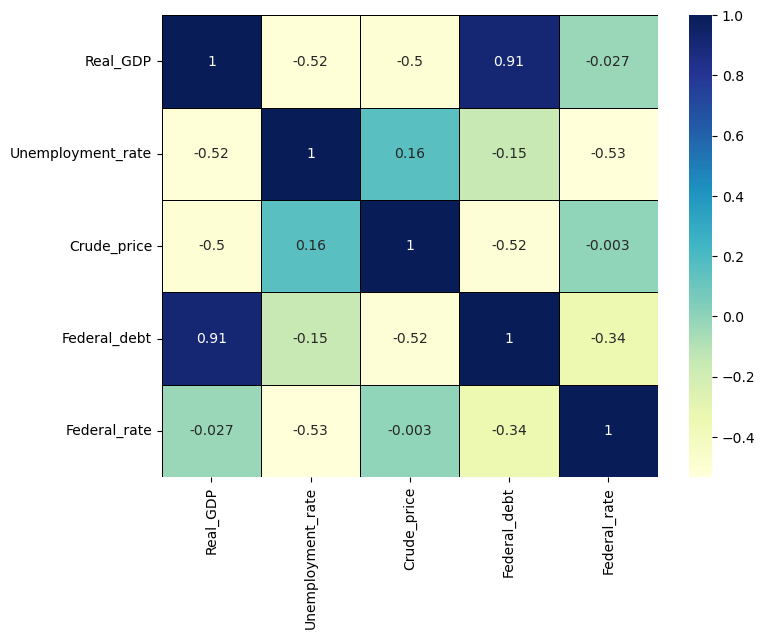
\includegraphics[width=\textwidth]{Latex Template/Englisch/img/Heatmap.png}
    \caption{Correlation matrix for macroeconomic variables used in regression}
    \hfill
\end{figure}

\begin{figure}[!h]
  \centering
    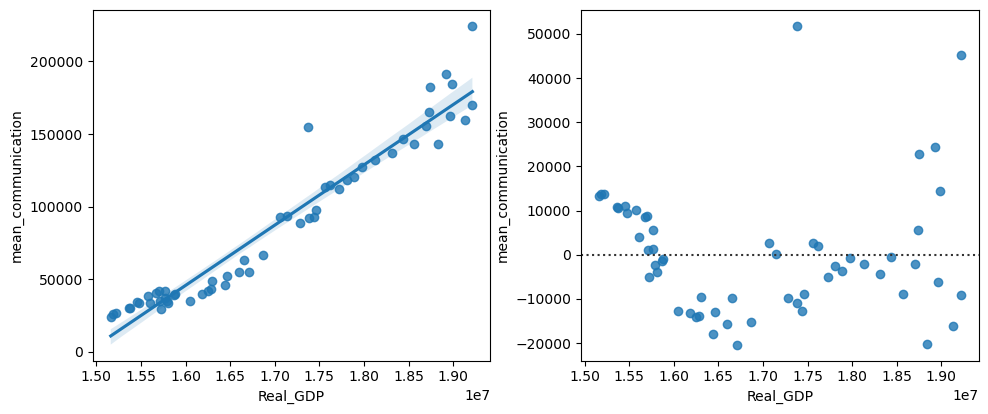
\includegraphics[width=\textwidth]{Latex Template/Englisch/img/Communication.png}
    \caption{Regression and residual plot Communication Services sector}
    \hfill
\end{figure}

\begin{figure}[!h]
  \centering
    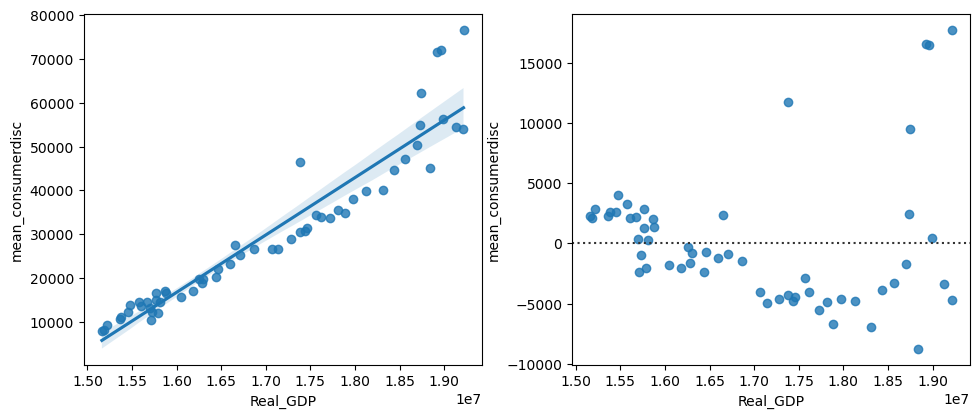
\includegraphics[width=\textwidth]{Latex Template/Englisch/img/Consumer Discreationary.png}
    \caption{Regression and residual plot Consumer Discretionary sector}
    \hfill
\end{figure}

\begin{figure}[!h]
  \centering
    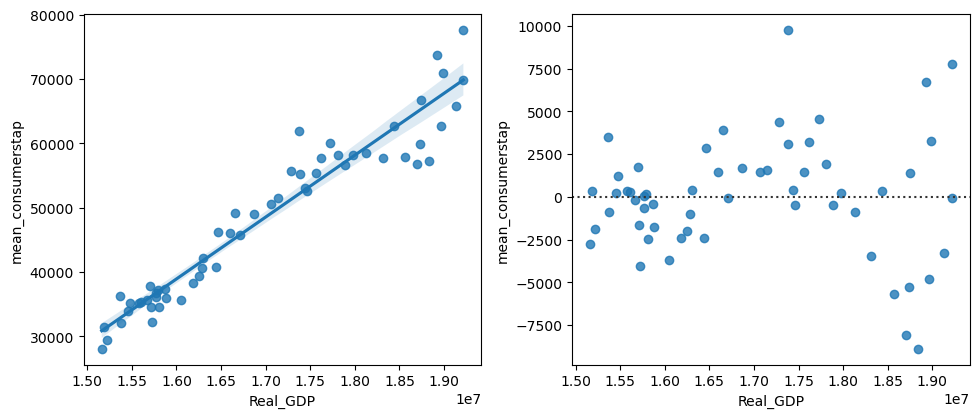
\includegraphics[width=\textwidth]{Latex Template/Englisch/img/Consumer Staples.png}
    \caption{Regression and residual plot Consumer Staples sector}
    \hfill
\end{figure}

\begin{figure}[!h]
  \centering
    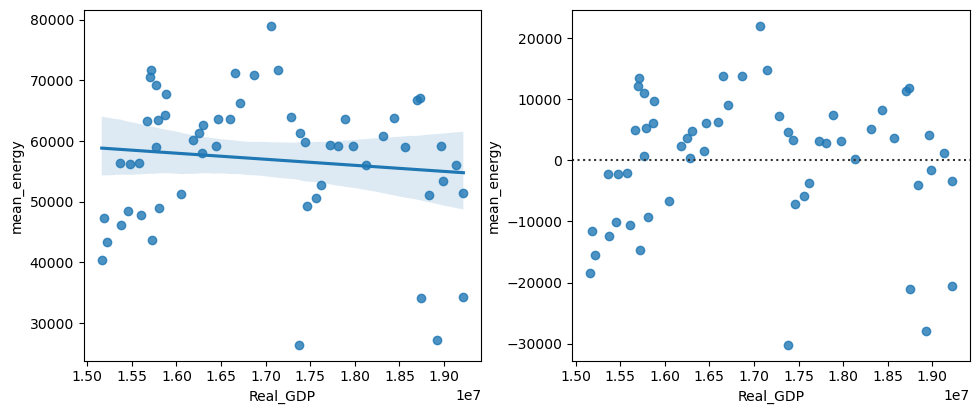
\includegraphics[width=\textwidth]{Latex Template/Englisch/img/Energy.png}
    \caption{Regression and residual plot Energy sector}
    \hfill
\end{figure}

\begin{figure}[!h]
  \centering
    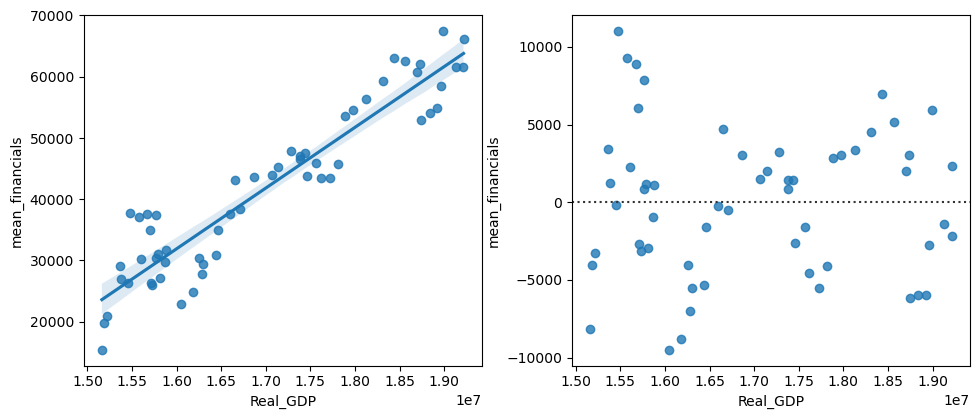
\includegraphics[width=\textwidth]{Latex Template/Englisch/img/Financials.png}
    \caption{Regression and residual plot Financials sector}
    \hfill
\end{figure}

\begin{figure}[!h]
  \centering
    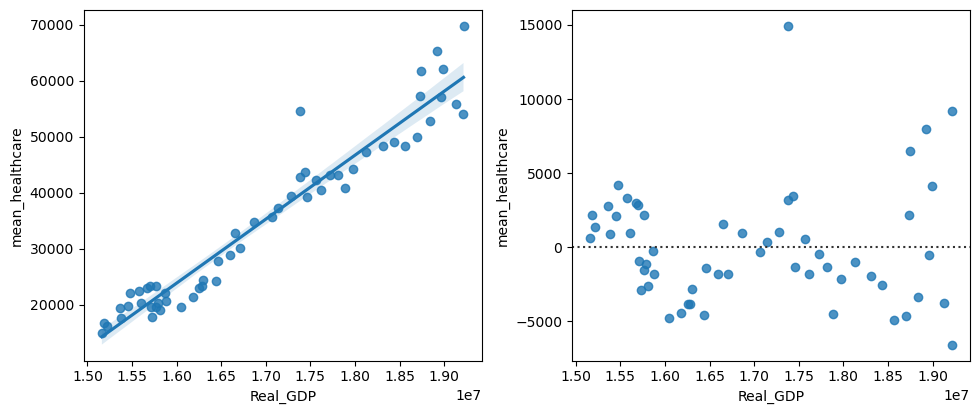
\includegraphics[width=\textwidth]{Latex Template/Englisch/img/Health Care.png}
    \caption{Regression and residual plot Health Care sector}
    \hfill
\end{figure}

\begin{figure}[!h]
  \centering
    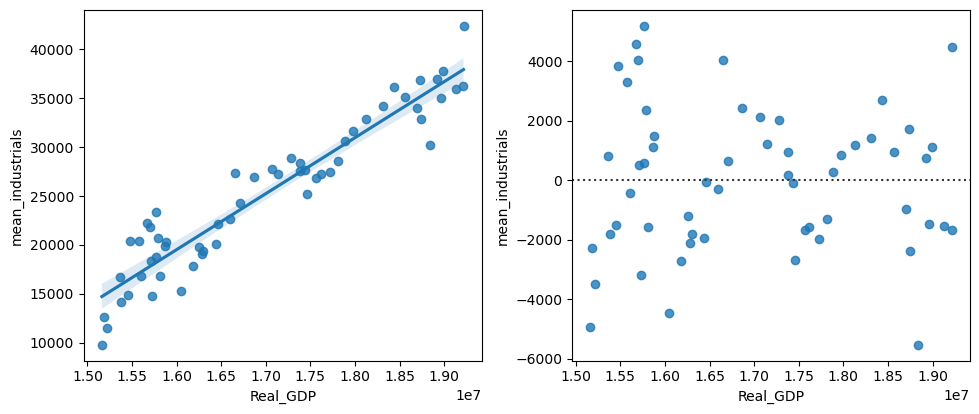
\includegraphics[width=\textwidth]{Latex Template/Englisch/img/Industrials.png}
    \caption{Regression and residual plot Industrials sector}
    \hfill
\end{figure}

\begin{figure}[!h]
  \centering
    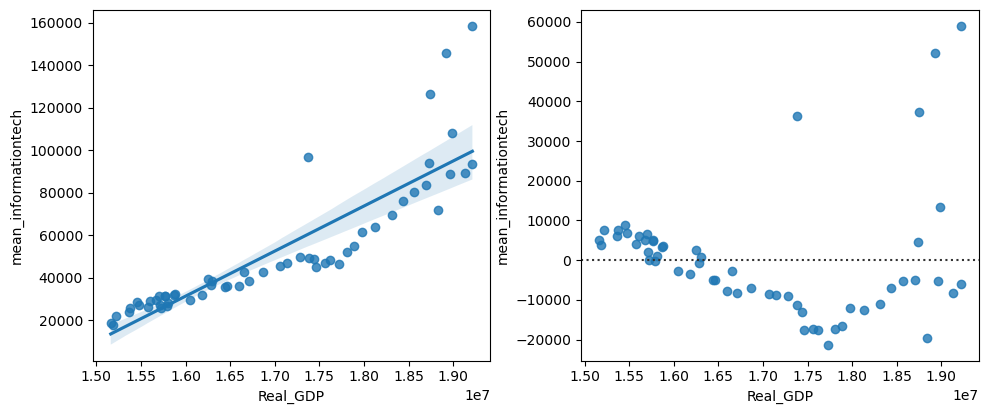
\includegraphics[width=\textwidth]{Latex Template/Englisch/img/IT.png}
    \caption{Regression and residual plot Information Technology sector}
    \hfill
\end{figure}

\begin{figure}[!h]
  \centering
    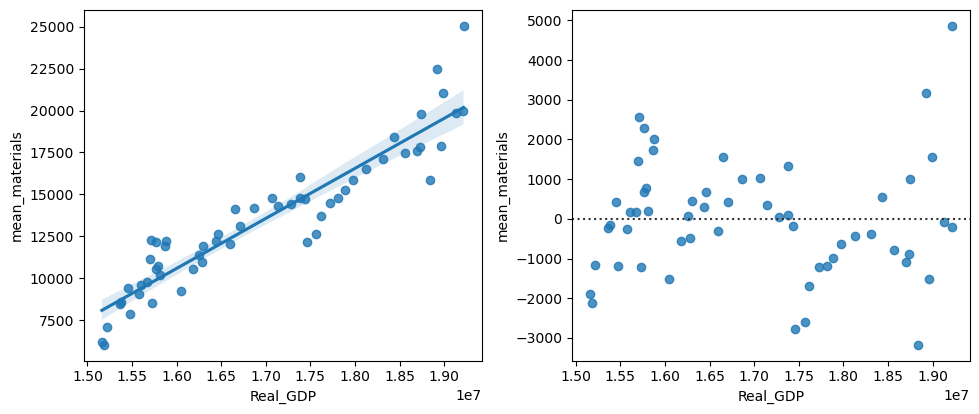
\includegraphics[width=\textwidth]{Latex Template/Englisch/img/Materials.png}
    \caption{Regression and residual plot Materials sector}
    \hfill
\end{figure}

\begin{figure}[!h]
  \centering
    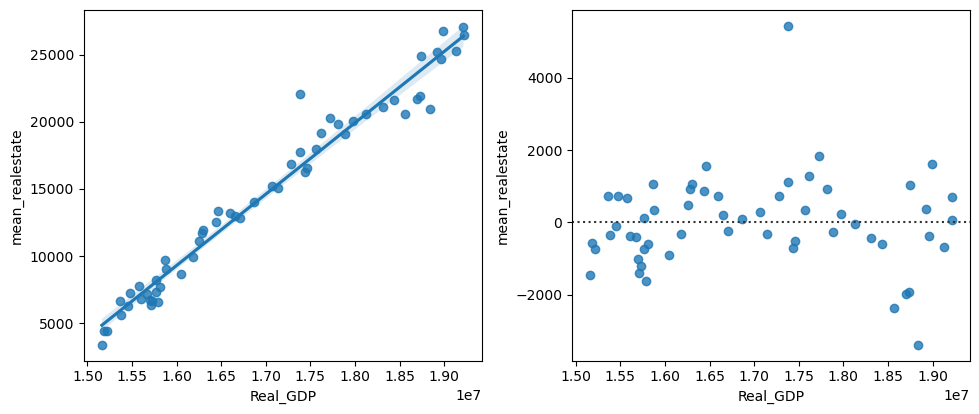
\includegraphics[width=\textwidth]{Latex Template/Englisch/img/Real Estate.png}
    \caption{Regression and residual plot Real Estate sector}
    \hfill
\end{figure}


\makeatletter
\setlength{\@fptop}{0pt}
\makeatother

 \begin{figure}[!h]
    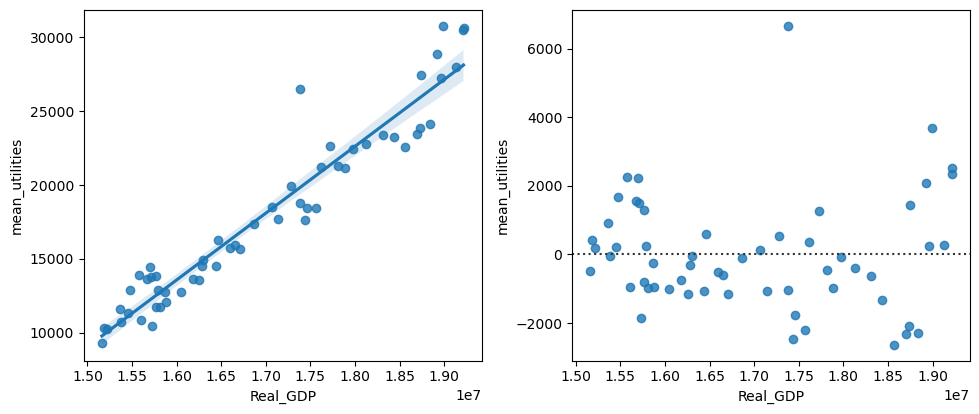
\includegraphics[width=\textwidth]{Latex Template/Englisch/img/Utilities.png}
    \caption{Regression and residual plot Utilities sector}
    \hfill
\end{figure}


\end{document}
